\documentclass{beamer}
\usepackage{TimosThesePresentation}
\usepackage{TimosTheseCommands}
\usepackage{TimosTheseInfo}


\title[\authorname{} M.Sc. Presentation]{A System for measuring Temperature dependent Surface Photovoltage}

\subtitle{by Timo Bretten}

\institute[\univname]{\univname}

\date[December 10th 2015]{M.Sc. Final Presentation December 10th 2015}

\begin{document}
\begin{frame}
  \titlepage
\end{frame}

\begin{frame}
  \frametitle{Outline}
  \tableofcontents
\end{frame}

\section{Introduction}
\begin{frame}
\frametitle{Some Background}
\begin{block}{About my M.Sc. project\dots}
\begin{minipage}{0.55\linewidth}
	\begin{itemize}
		\item Research carried out in 13/14 at \deptname{}
		\item Project had two parts: \pvdf{} \& \spv{}(T)
		\item Only part two will be presented
	\end{itemize}
\end{minipage}
\hfill
\begin{minipage}{0.4\linewidth}
\centering
	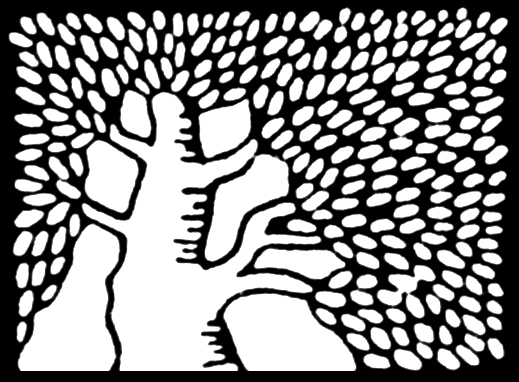
\includegraphics[width=1\linewidth]{./figs/logos/weiz}
\end{minipage}
\end{block}\end{frame}

\begin{frame}
\frametitle{Motivation}
\begin{block}{The goal of this project is to\dots}
	\begin{itemize}
		\item verify results from a \enhyphen{new} experimental set up against established systems
		\item expand the capabilities of the \enhyphen{new} set up
		\item ultimately measure temperature dependent \spv{}
	\end{itemize}
\end{block}\end{frame}

\section{Theory}
\begin{frame}
\frametitle{Physical Causes of \cpd{} \& \spv{}}
\begin{block}{The Kelvin Probe}
\begin{minipage}{0.55\linewidth}
	$\begin{array}{l l}
		\cpd{} &\equiv \wfp - \wfs \\
		C(t) &= \frac{\epsilon \epsilon_0 A}{d(t)} \\
		I(t) &= \frac{dQ}{dt}= (\cpd{}+V_b) \frac{dC}{dV} \\
		I(\Delta V) &= -\epsilon \epsilon _0 A (\cpd{}+V_b) \, f(\omega t)
	\end{array}$
\end{minipage}
\hfill
\begin{minipage}{0.4\linewidth}
\centering
	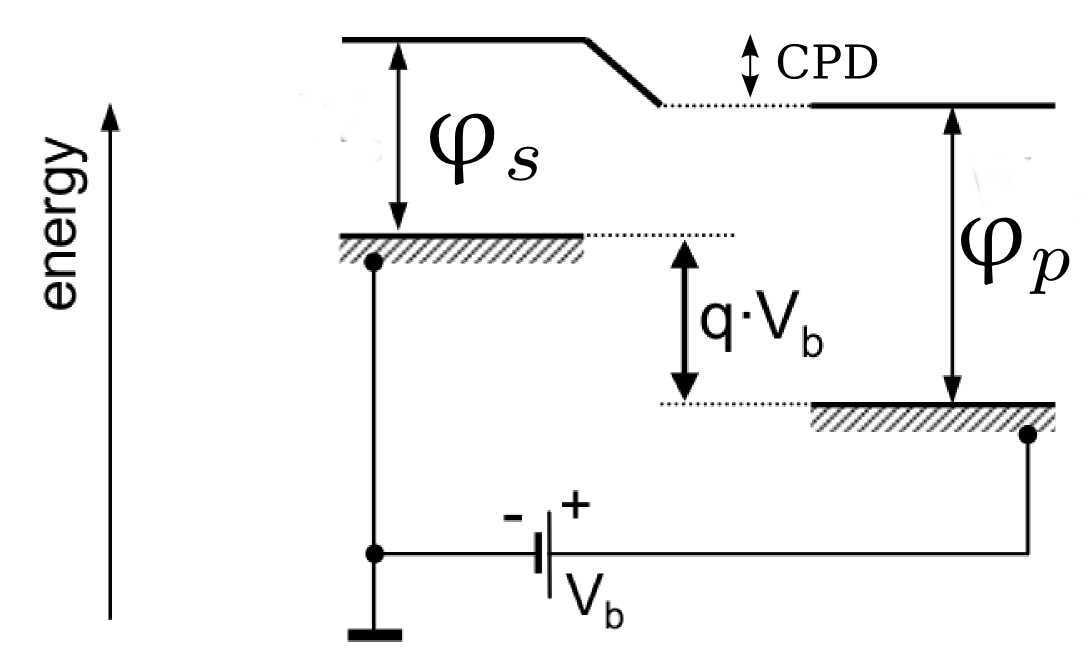
\includegraphics[width=1\linewidth]{./figs/pres/kp-scheme}\\
	\textcolor{RUred}{[1]}
\end{minipage}
\end{block}\end{frame}

\begin{frame}
\frametitle{Physical Causes of \cpd{} \& \spv{}}
\begin{block}{Band bending \& \spv{}: dark vs. light}
\centering
$\text{\spv} \equiv \cpd_{\text{light}} - \cpd_{\text{dark}}$\\[-8pt]\hrulefill\\[-5pt]
\begin{minipage}{0.45\linewidth}
\centering
	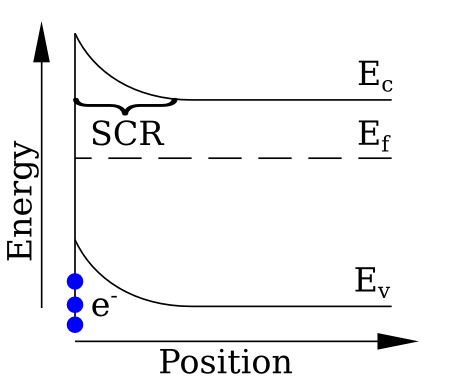
\includegraphics[width=1\linewidth]{./figs/pres/bb-dark}
\end{minipage}
\hfill
\begin{minipage}{0.45\linewidth}
\centering
	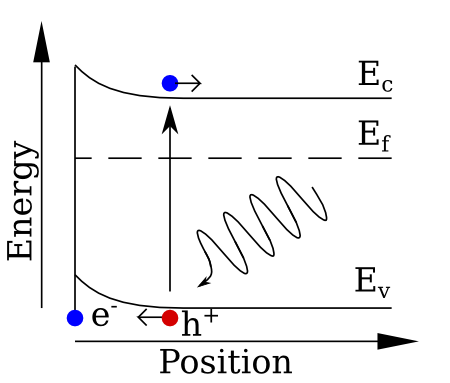
\includegraphics[width=1\linewidth]{./figs/pres/bb-light}
\end{minipage}
\end{block}\end{frame}

\begin{frame}
\frametitle{Physical Causes of \cpd{} \& \spv{}}
\begin{block}{Band bending \& \spv{}: n-type vs. p-type}
\centering
$\text{\spv} \equiv \upvarphi _{\text{s,dark}} - \upvarphi _{\text{s,light}}$\\[-8pt]\hrulefill\\[-5pt]
\begin{minipage}{0.45\linewidth}
\centering
	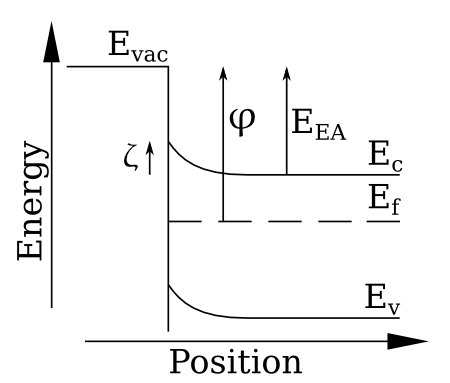
\includegraphics[width=0.9\linewidth]{./figs/pres/bbdefn}
\end{minipage}
\hfill
\begin{minipage}{0.45\linewidth}
\centering
	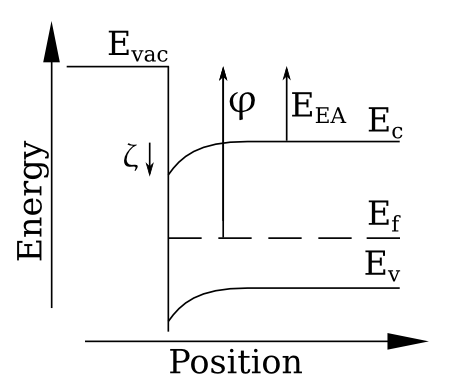
\includegraphics[width=0.9\linewidth]{./figs/pres/bbdefp}
\end{minipage}\\\hrulefill\\
$\text{\spv}_{\text{n-Type}} 	> 0	\qquad	\text{\spv}_{\text{p-Type}} 	< 0	$
\end{block}\end{frame}

\begin{frame}
\frametitle{Choosing a Model System}
\begin{block}{Metal Insulator Transition in \vadiox{}}
\begin{minipage}{0.5\linewidth}
	\begin{itemize}
		\item metal at $T>T_{MI}$
		\item semiconductor at $T<T_{MI}$
		\item insulator at $T \ll T_{MI}$
		\item Influences of W-doping:
		\begin{itemize}
			\item $T_{MI}\approx \SI{270}{\kelvin}$ \hspace{0.15cm} \textcolor{RUred}{[2]}
			\item $\upvarphi \phantom{_{MI}} \approx  \SI{5.15}{\electronvolt}$ \textcolor{RUred}{[3]}
		\end{itemize}
	\end{itemize}
\end{minipage}
\hfill
\begin{minipage}{0.45\linewidth}
\centering
	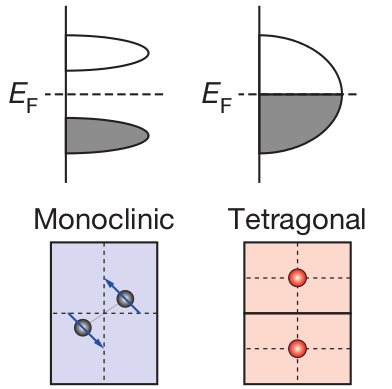
\includegraphics[width=1\linewidth]{./figs/pres/vo2gapopening}\\
	\textcolor{RUred}{[4]}
\end{minipage}
\end{block}\end{frame}

\section{The Systems}
\begin{frame}
\frametitle{Established \kp{} Systems}
\begin{block}{Ambient \& Glovebox \kp{}s}
\centering
\begin{minipage}{0.55\linewidth}
\centering
\begin{itemize}
	\item Besocke \kp{} head \& controller
	\item Humidity controlled ambient
	\item Glovebox ($<\num{5}$ppm \oxy{} \& \water{})
	\item Xenon lamp \& VariAC ($\sim$\SI{80}{\watt})
	\item Illumination is source of heat!
\end{itemize}
\end{minipage}
\hfill
\begin{minipage}{0.4\linewidth}
\centering
	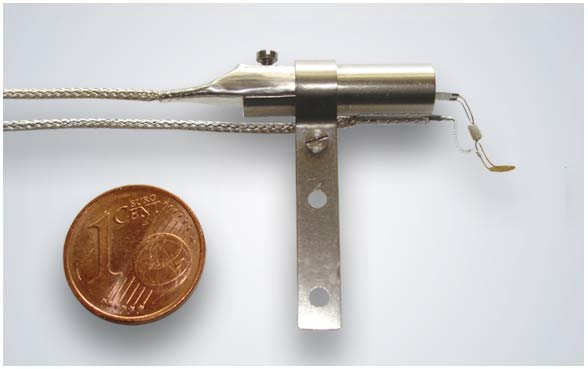
\includegraphics[width=1\linewidth]{./figs/pres/besocke}\\
	\textcolor{RUred}{[5]}
\end{minipage}
\end{block}\end{frame}

\begin{frame}
\frametitle{Cryogenic System with a \kp{}}
\begin{block}{Lakeshore with \McA{} \& \led{}}
\centering
\begin{minipage}{0.45\linewidth}
\centering
	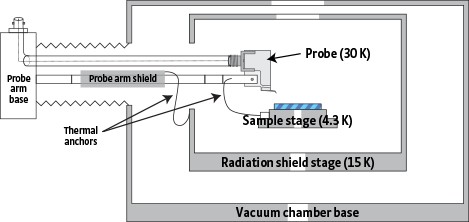
\includegraphics[width=1\linewidth]{./figs/pres/Config_TTPX}
\end{minipage}
\hfill
\begin{minipage}{0.45\linewidth}
\centering
	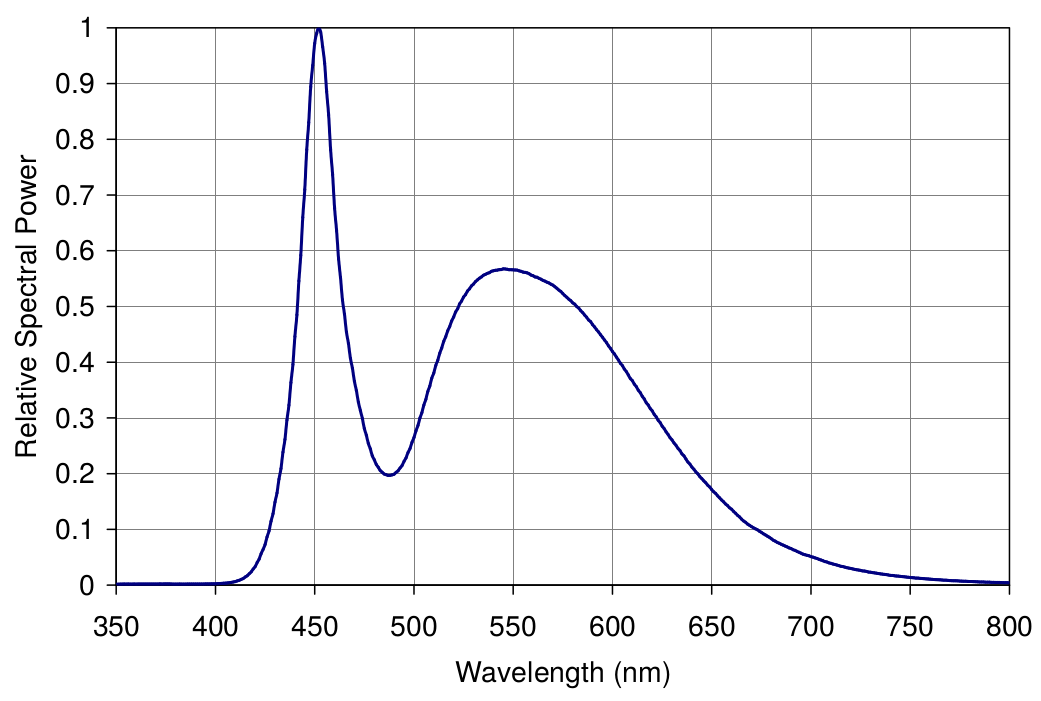
\includegraphics[width=1\linewidth]{./figs/pres/ledspec}
\end{minipage}\\
\hspace{0.25\linewidth}\textcolor{RUred}{[6]}\hfill\textcolor{RUred}{[7]}\hspace{0.2\linewidth}
\end{block}\end{frame}

\section{Experimental}
\begin{frame}
\frametitle{Checking against Established Systems}
\begin{block}{Behaviour at Room Temperature}
\centering
\begin{minipage}{0.45\linewidth}
\centering
	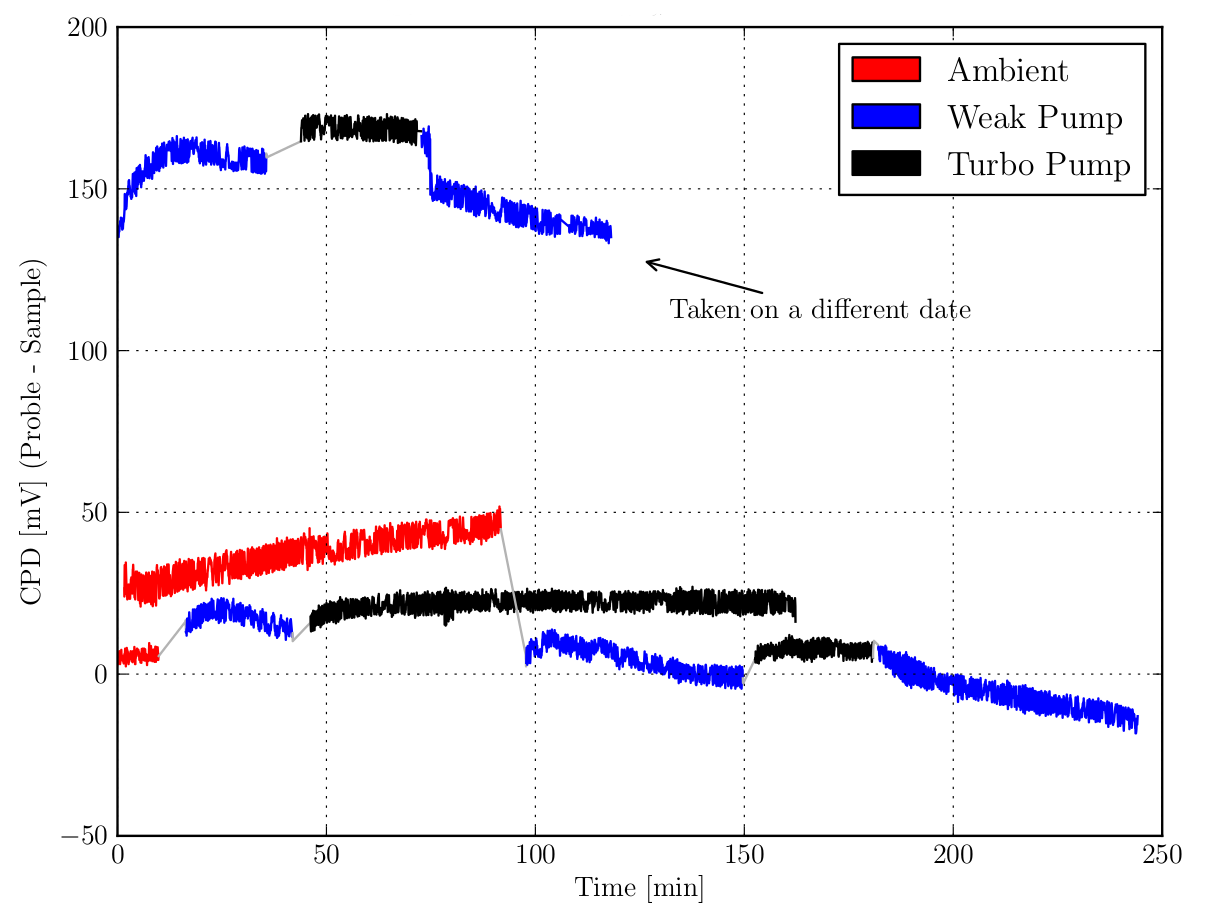
\includegraphics[width=1\linewidth]{./figs/pres/HOPGMcA}
\end{minipage}
\hfill
\begin{minipage}{0.45\linewidth}
\centering
	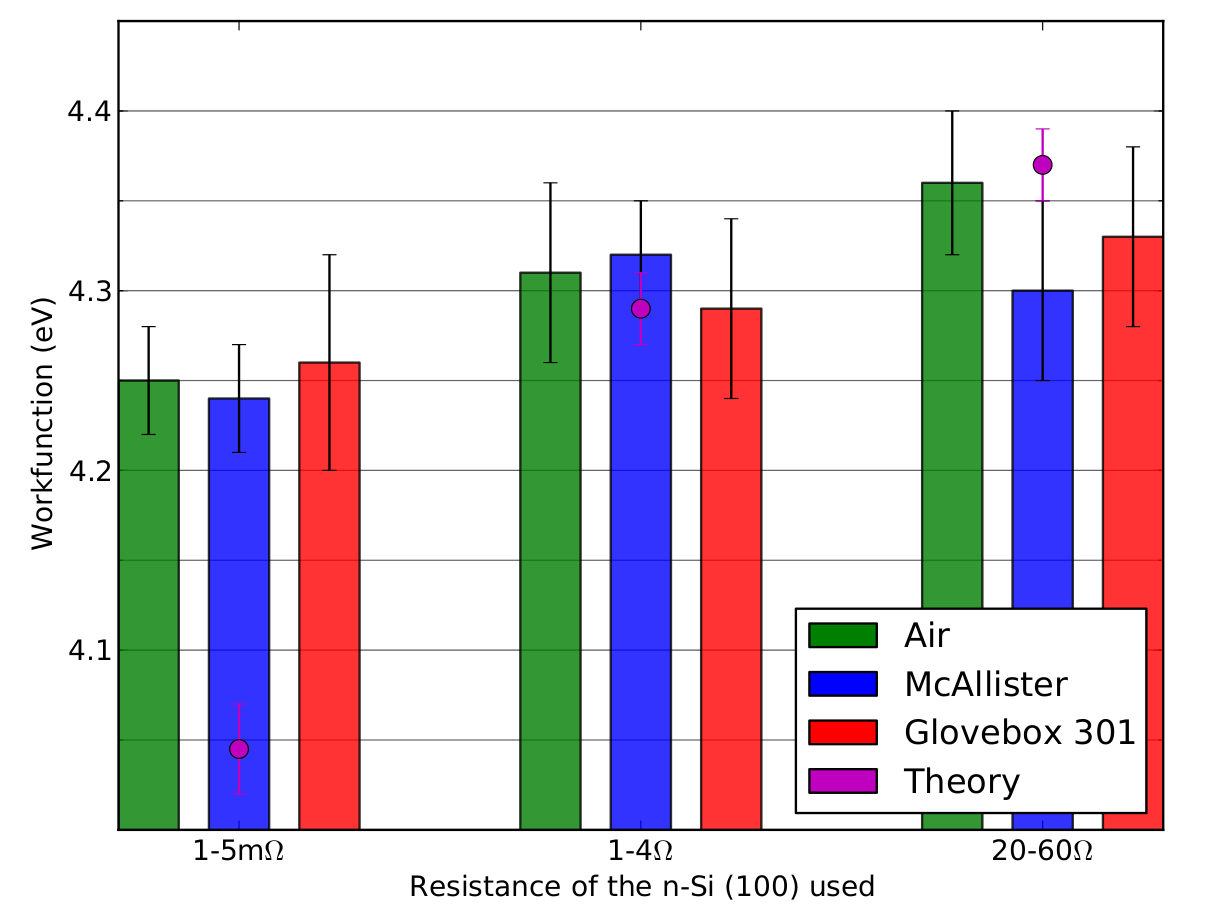
\includegraphics[width=1\linewidth]{./figs/pres/Sih}
\end{minipage}\\[5pt]\hrulefill\\
\enhyphen{Jumps} probably due to movement of probe head\\
Excellent agreement between systems
\end{block}\end{frame}

\begin{frame}
\frametitle{Checking against Established Systems}
\begin{block}{Behaviour at lower temperatures and \spv{}}
\centering
\begin{minipage}{0.4\linewidth}
	\begin{itemize}
		\item $\upvarphi_{\text{Alumina}}$ at \SI{300}{\kelvin}: \SI{4.00+-0.12}{\electronvolt}
		\item $\upvarphi_{\text{Alumina}}$ at \SI{250}{\kelvin}: \SI{4.17+-0.15}{\electronvolt}
	\end{itemize}
\end{minipage}
\hfill
\begin{minipage}{0.55\linewidth}
\centering
	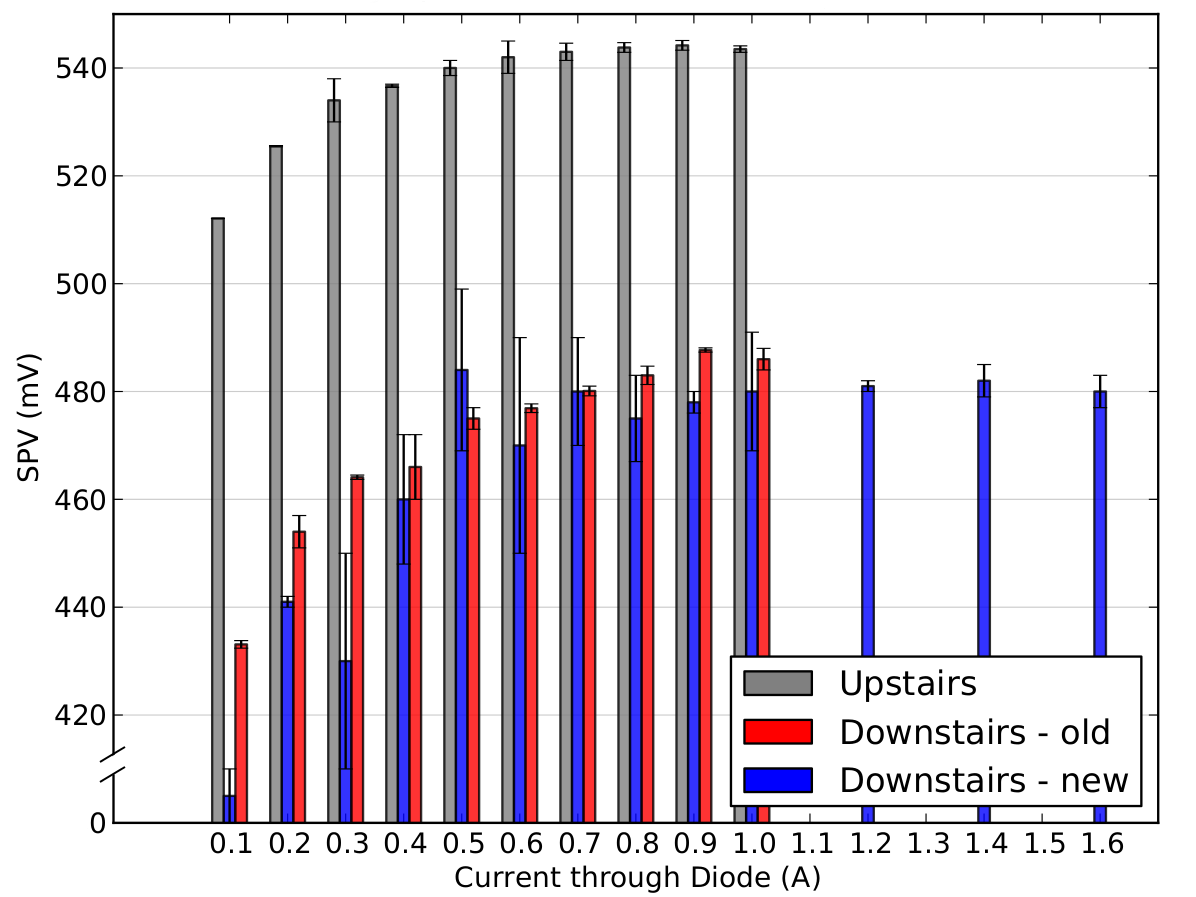
\includegraphics[width=1\linewidth]{./figs/pres/currentseries}
\end{minipage}\\[5pt]\hrulefill\\
Probably no ice, even on very hydrophilic surface\\
\spv{} $\sim$\SI{12}{\percent} too low. Shadows on the sample?
\end{block}\end{frame}

\begin{frame}
\frametitle{Temperature Dependent \cpd{} in \wvadiox{}}
\begin{block}{Temperature Sweep and precise Measurement}
\centering
\begin{minipage}{0.45\linewidth}
\centering
	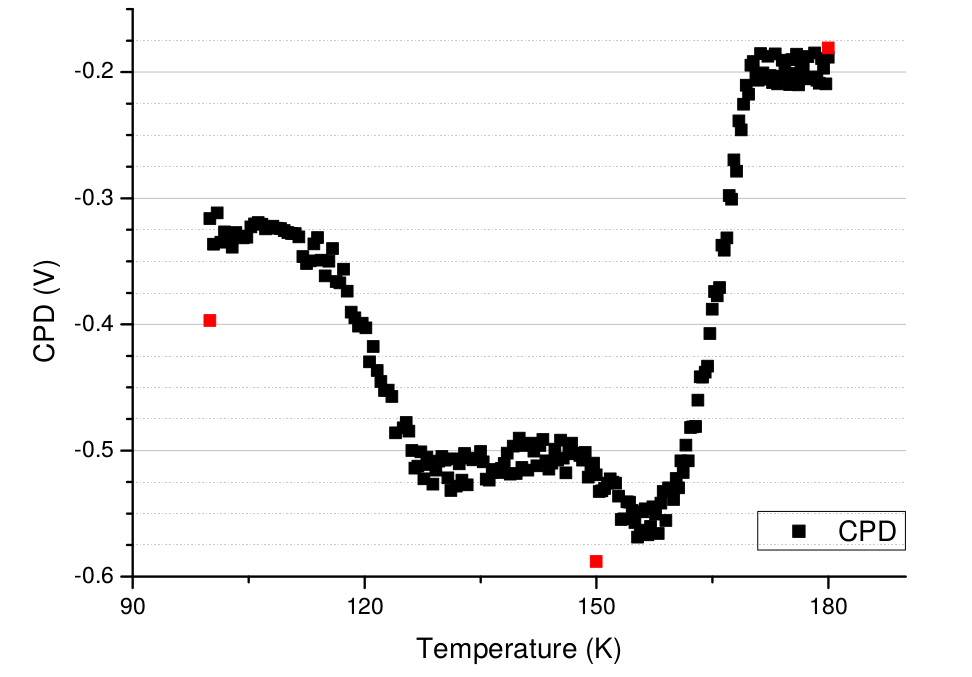
\includegraphics[width=1\linewidth]{./figs/pres/vox1pres}
\end{minipage}
\hfill
\begin{minipage}{0.45\linewidth}
\centering
	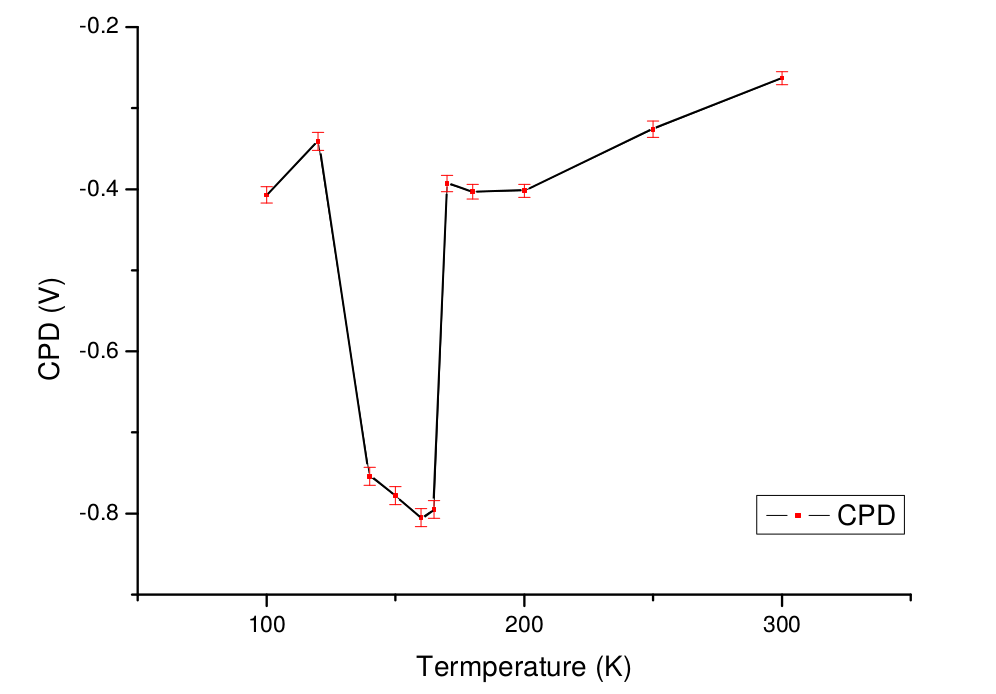
\includegraphics[width=1\linewidth]{./figs/pres/vox2pres}
\end{minipage}\\[5pt]\hrulefill\\
Curious behaviour in the range \SIrange{120}{160}{\kelvin}, far below $T_{MI}$ \\
Effect of substrate?
\end{block}\end{frame}

\begin{frame}
\frametitle{Temperature Dependent \spv{} in \wvadiox{}}
\begin{block}{$\rho$(T) and \spv{}(T)}
\centering
\begin{minipage}{0.45\linewidth}
\centering
	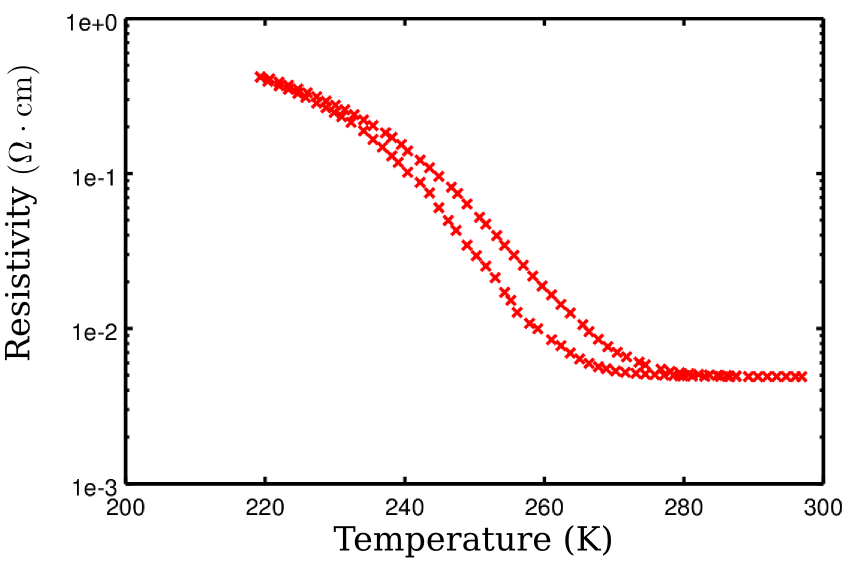
\includegraphics[width=1\linewidth]{./figs/pres/vo2resis}\\
	{\small Measurement by Nir Kedem}
\end{minipage}
\hfill
\begin{minipage}{0.45\linewidth}
\centering
	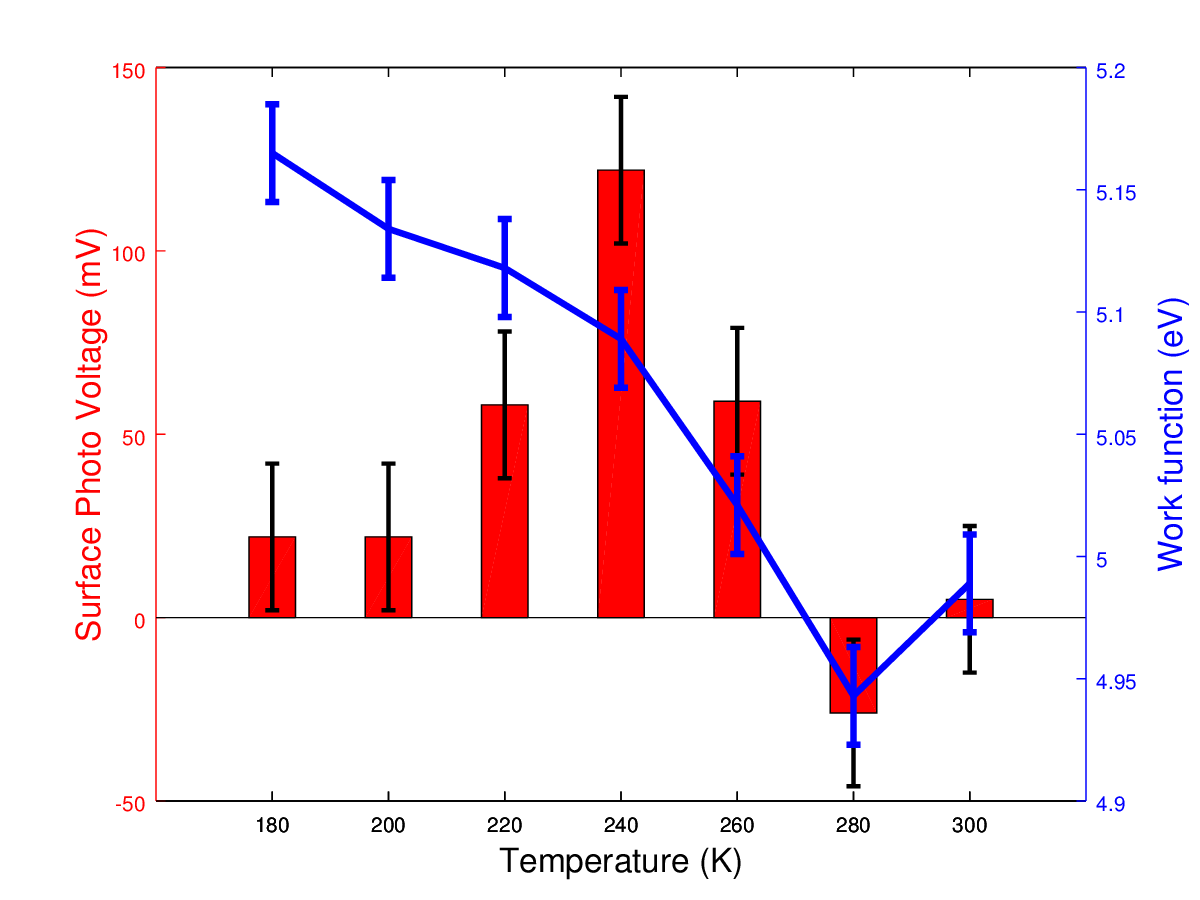
\includegraphics[width=1\linewidth]{./figs/pres/vox3}\\
	\phantom{{\small Measurement by Nir Kedem}}
\end{minipage}\\[5pt]\hrulefill\\
\spv{} identifies \wvadiox{} as n-type material\\
Appearance of \spv{} and change in \wf{} in accordance with resistivity and literature \textcolor{RUred}{[2,3]}
\end{block}\end{frame}
\section{Discussion \& Conclusion}
\begin{frame}
\frametitle{Discussion \& Conclusion}
\begin{block}{We showed that\dots}
\centering
\begin{itemize}
	\item \cpd{} is in excellent agreement with established systems
	\item \spv{} $\sim$\SI{12}{\percent} too low. Shadowing?
	\item \cpd{}(T) reproducible and interesting
	\item \spv{}(T) shows expected behaviour for model system
	\item[$\rightarrow$] Lakeshore + \McA{} + \led{} is a viable system for \spv{}(T)
\end{itemize}
\end{block}\end{frame}

\begin{frame}
\frametitle{List of References}
\begin{block}{Literature and links}
\centering
	\begin{tabular}{r l}
	\textcolor{RUred}{[1]} & \href{https://www.helmholtz-berlin.de/media/media/forschung/energie/heterogen/eta/methods/spv-techniques-2010-08-09.pdf}{SPV Technique, Helmholtz Institute Berlin}\\
	\textcolor{RUred}{[2]} & Changhyun Ko~\etal{} \emph{ACS Appl. Mater. Interfaces}, \\
	& 3(9):3396-3401, 2011\\
	\textcolor{RUred}{[3]} & Keisuke Shibuya~\etal{}. \emph{Phys Rev. B}, 82(20), 2010 \\
	\textcolor{RUred}{[4]} & M. Nakano~\etal{}. \emph{Nature}, 487(7408):459-462, 2012 \\
	\textcolor{RUred}{[5]} & \href{http://www.besocke-delta-phi.de/kelvin.htm}{Besocke Website} \\
	\textcolor{RUred}{[6]} & \href{http://lakeshore.com/products/cryogenic-probe-stations/
model-ttpx-cryogenic-probe-station/pages/Overview.aspx}{Lakeshore Website} \\
	\textcolor{RUred}{[7]} & \href{http://www.ledengin.com/files/products/LZP/
LZP-00CW0R.pdf}{LEDengine Website}
	\end{tabular}
\end{block}\end{frame}

\begin{frame}
\frametitle{Acknowledgements}
\begin{block}{Thanks! to\dots}
\centering
	\begin{tabular}{r l}
	\textcolor{RUred}{Prof. Dr. David Cahen} & for his supervision \\
	\textcolor{RUred}{Dr. Hugo Meekes} & for his spontaneous support \\
	\textcolor{RUred}{Igal Levin} & for keeping me (somewhat) on track \\
	\textcolor{RUred}{Nir Kedem} & for always having an answer
	\end{tabular}
\end{block}\end{frame}
\end{document}